\chapter{Drifter analysis}\label{ch:drifters}
\section{Introduction}

While previous chapters provided information about the shelf
circulation in small quasi-synoptic time scales, this chapter will
focus on the Lagrangian observations of the regional behaviour of
mixed-layer drifters. The study of the upper layer circulation
with surface mixed-layer drifters has become a very attractive
option due to its broad scaling sampling capabilities and low
cost. As they inherently average over space and time, they are
well suited for measuring the large-scale, low-frequency field
that produces the diffusive transport. Nonetheless, drifters are
``quasi-Lagrangian'' because they can not follow vertical
displacements. This becomes particularly relevant in the presence
of flow inhomogeneities.

Mixed-layer drifters have been successfully used to track the
complex mesoscale circulation associated with Eastern Upwelling
Systems \citep{Brink91b,Brink00}. In the California Upwelling
System their capability to follow jets associated with upper layer
fronts has been demonstrated \citep[e.g.][]{Swenson92}. They have
also been useful in the study of upper flow dynamics
\citep[e.g.][]{Flament00} and even high frequency motions like the
upper layer inertial response to wind forcing \citep{Poulain90}.
Drifters Lagrangian statistics have also proved important in
evaluating model performance at large scales \citep{McClean02}.

The large volume of drifter data collected to date has enabled the
development of statistical techniques to estimate horizontal
mixing coefficients from drifters \citep[e.g.][]{Colin83,Davis85}.
These studies have helped characterize the diffusive properties of
oceanic regions and to validate the representation of oceanic
mixing in numerical models. Estimates have ranged from basin scale
studies \citep[e.g.][]{Fratantoni01} to more regional studies
\citep{Dever98,Poulain01}.

The diffusive properties of the drifters can  be related to the
scales of motion of the random velocity field \citep{Swenson96}
and can be used to evaluate the predominant mesoscale field that
distributes energy, momentum and heat. \citet{Davis85} showed that
large open ocean mesoscale eddies (with Lagrangian space and time
scales of L$\sim$50-100 km and T$\sim$10 days) displayed larger
horizontal diffusivities (K$\sim 10^7$\mixc) than the smaller
coastal eddies (L$\sim$30 km, T$\sim$1-2 days and K$\sim
10^{4-6}$\mixc).

Previous mixed-layer drifter deployments in the present study area
included those described by \citet{Haynes91} and during the MORENA
EU project \citep{Martins02}. They focused on the setup and
evolution of the winter poleward flow (e.g.
Chapter~\ref{ch:winter}) while here, two contrasting seasonal
regimes are compared. Other drifter releases in the region have
concentrated in the seeding and tracking of swoddies (Slope Water
Oceanic Eddies) \citep{Pingree92} or have studied deeper levels
\citep[the French ARCANE program,][]{Paillet02}.

A quantitative description of the regional Lagrangian statistics
and their seasonal variability within the Galician region is
provided by 2 sets of 4 satellite tracked drifters released in the
OMEX area in August of 1998 (``summer deployment'') and January
1999 (``winter deployment''). The exact deployment date and
location are summarised in table~\ref{tb:drf_deploym}. The total
number of drifter days was 822 (478 during the ``summer
deployment'' and 344 for the ``winter'' one). This is the first
time diffusivity estimates have been calculated during the Iberian
upwelling regime even if with a limited number of drifters.

\begin{table}[ht]
  \centering
\begin{tabular}{rccccccr}
\hline \hline
& \multicolumn{3}{c}{ Launch } & \multicolumn{3}{c}{End of Record}\\
\cline{1-8} { I.D.  } & Date  & Latitude  & Longitude &
Date & Latitude & Longitude & Days  \\
\cline{1-8} %
10312&12/08/98&41\deg58.31&9\deg47.06&05/03/99&38\deg00.50&12\deg28.68&205\\
10313&12/08/98&41\deg53.83&9\deg47.29&25/11/98&41\deg50.34&10\deg49.20&103\\
10314&12/08/98&41\deg53.82&9\deg52.89&05/12/98&36\deg59.4&13\deg29.94&110\\
10315&12/08/98&41\deg58.71&9\deg53.10&13/10/98&40\deg23.10&12\deg12.06&60\\
4010&02/01/99&40\deg59.97&9\deg24.86&17/05/99&38\deg43.50&9\deg36.90&134\\
3924&02/01/99&40\deg59.98&9\deg27.72&17/05/99&38\deg00.24&10\deg48.36&82 \\
4558&02/01/99&41\deg01.85&9\deg27.83&08/04/99&39\deg21.18&9\deg22.62&95\\
3923&02/01/99&41\deg01.91&9\deg25.37&05/02/99&42\deg54.36&9\deg15.66&33\\
\hline \hline
\end{tabular}
  \caption{Summary of each of the drifters releases. Latitude in degrees North
  and Longitude in degrees West.}\label{tb:drf_deploym}
\end{table}

\section{Data and methods}
\begin{figure}
\centering \arribacap
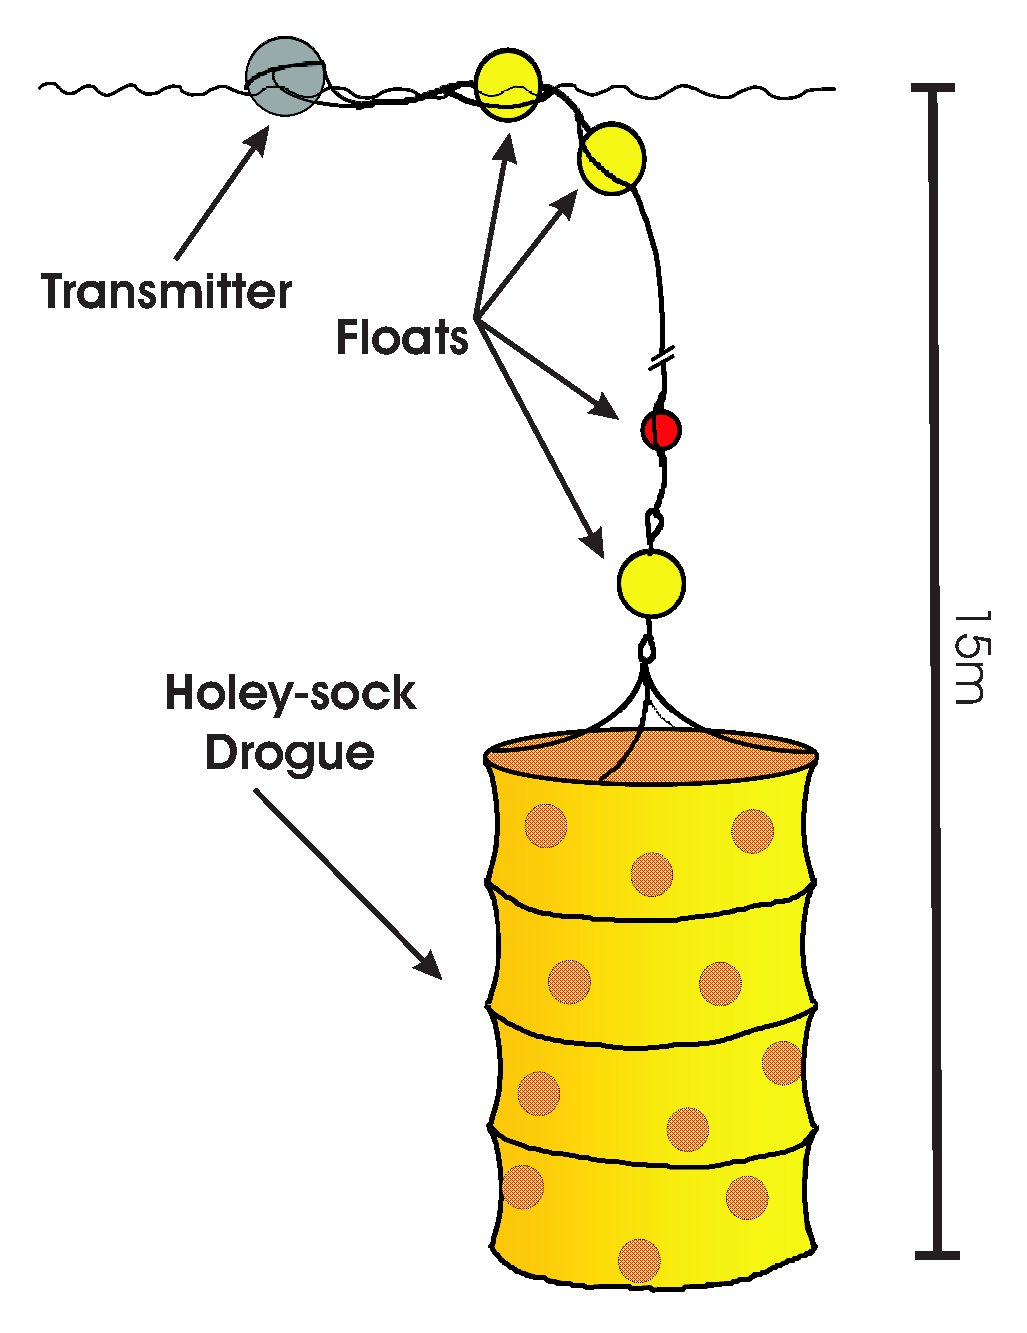
\includegraphics[width=8cm]{buoy_design}%
\caption{Standard drifter design used in this work. The spherical
transmitter corresponds to the SERPE-IESM model.} %
\label{fig:drf_design}
\end{figure}
All drifters deployed for this study carried a Holey-sock drogue
at a nominal depth of 15m (Fig~\ref{fig:drf_design}) as described
in Chapter~\ref{ch:summer}. The subsurface buoyancy provides
decorrelation of the surface float from surface waves induced high
frequency motion in the drogue,  and allowing the satellite
transmitter to remain above the surface water. The transmitter was
different in the two deployments. In the ``summer'' release
cylindrical Horizon Marine Inc units were used while spherical
SERPE-IESM transmitters were used during the ``winter'' one. Both
configurations were tracked through the ARGOS system yielding 6-8
fixes a day (Fig.~\ref{fig:drf_classes}). The ARGOS positioning
system supplies an accuracy flag divided in 4 classes, 0, 1, 2 and
3. The first class has no upper limit in its accuracy and they
were removed from the data. Classes 1, 2 and 3 correspond to
accuracies of 1000-350m, 350-150m and less than 150m respectively.
Typical examples for one ``summer'' and one ``winter'' drifter are
presented in Fig~\ref{fig:drf_classes} as 5 day bins histograms.
Global average percentages were 39\%, 43\% and 18\% for classes 1,
2 and 3. There were indications of a larger number fixes during
the ``winter'' deployment than the ``summer'' one probably related
to the larger floatability of the SERPE-IESM spherical drifter.
\begin{figure}
\centering \arribacap \subfigure[]{
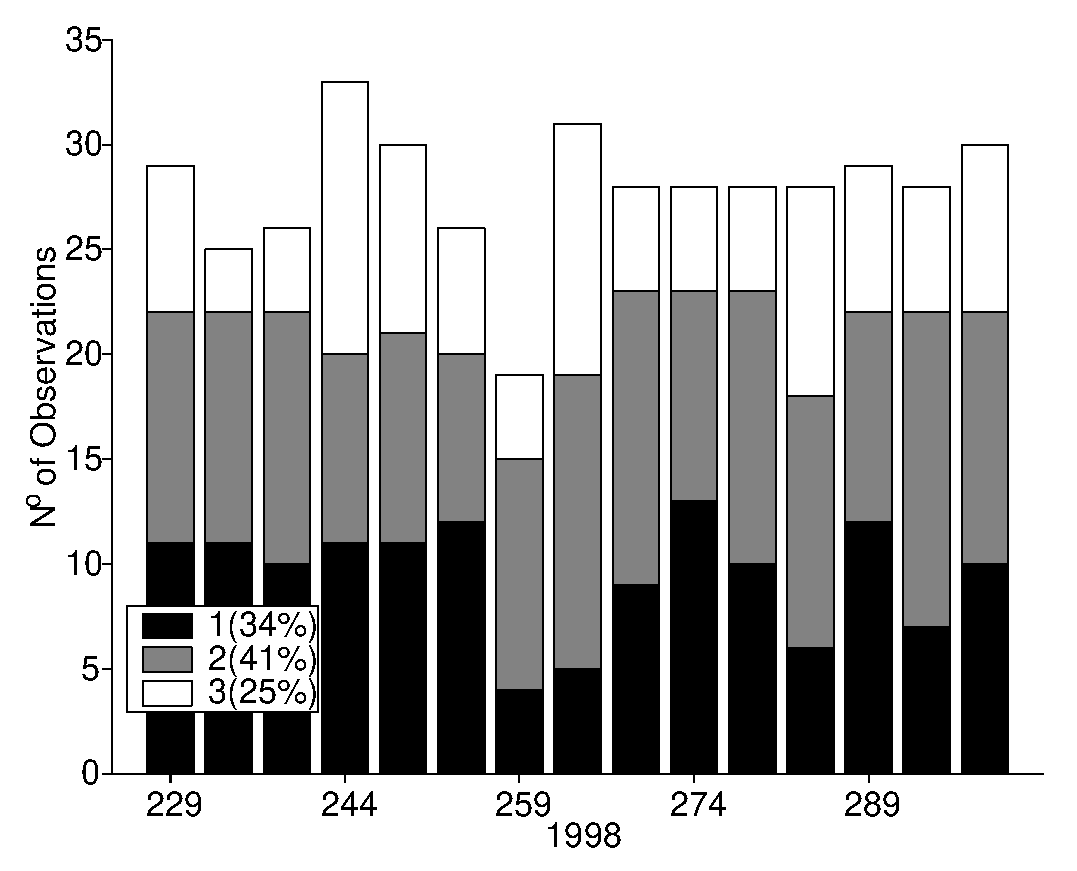
\includegraphics[width=6.5cm]{hist10312}}%
\subfigure[]{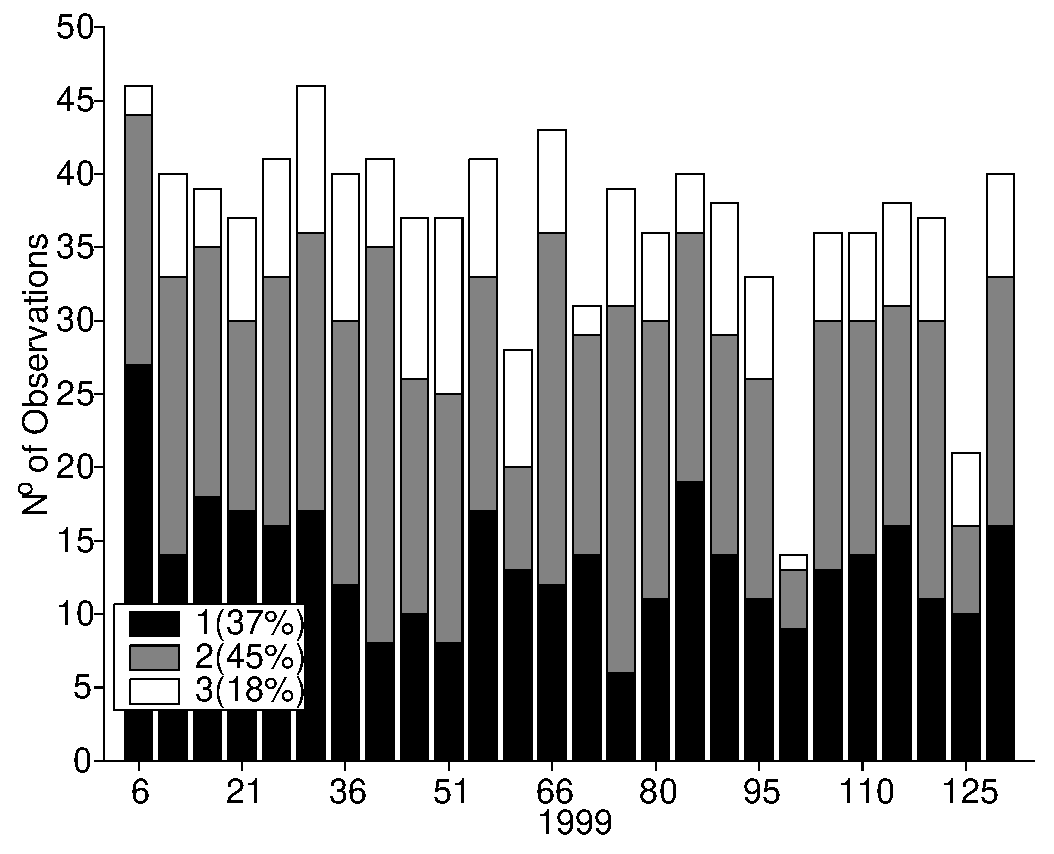
\includegraphics[width=6.5cm]{hist04010}}%
\caption{Examples of 5 day bins histogram distribution of location
classes for drifters 10312 and 04010 during part of the ``summer''
and ``winter'' deployment respectively. Note average number of
fixes in a) is 5-6 while it increases in b) to 7-8.}
\label{fig:drf_classes}
\end{figure}

All drifters were screened for evidences of drogue loss through a
sustained increase in the velocity variance of the raw data
similarly to \citet{Burrows99} and none were found. In fact, two
``winter'' drifters ( I.D. 3923 and 4558) grounded after 95 and 33
days respectively and both were recovered with the drogue still
attached.

All drifter data have been regularly interpolated to 1 hour
intervals with a cubic spline (NAG routines E01BAF and E02BBF).
Gaps larger than 6 hours were linearly interpolated prior to the
use of the cubic spline. Velocity estimates were generated by
taking the first derivative of the cubic-spline. The data were
then filtered with a 60+1+60 Cosine-Lanczos filter with a half
power point at 40hours and subsampled at 6 hours intervals
\citep{Haynes91}. This way, the data were efficiently removed of
any periodicity longer than 40 hours (tidal and inertial currents,
Fig~\ref{fig:drf_filter}), hence avoiding aliasing the energy into
the low frequency motions that are of primary interest here.
Nevertheless, frequency analysis of the drifter data set showed
the inertial-band wave energy at this latitude range to be
generally low. Complex demodulation of the velocity time series
around the inertial frequency yielded amplitudes in the order of
2-5\velc, smaller than the velocities associated with the
structures responsible for the residual flow, upwelling
front-filaments (20-35\velc) or the winter poleward flow
(15-25\velc). Similarly, in other regions situated at the same
latitude, e.g. in the California Current, the inertial band energy
is at least 1 order of magnitude less than the low-frequency
motions energy \citep{Swenson96}.


\begin{figure}
\centering \arribacap
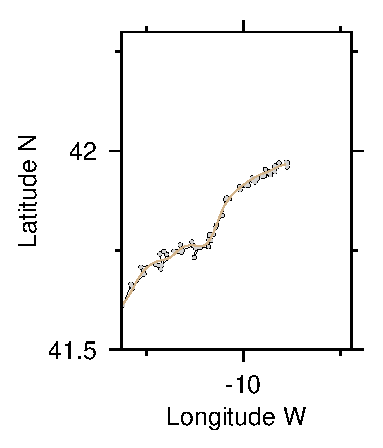
\includegraphics[width=6.5cm]{unfilt_drifter}%
\caption{Filtered and raw data of drifter 10312
during the first 10 days of deployment.} %
\label{fig:drf_filter}
\end{figure}


\subsection{The Summer deployment}
\begin{figure}
\centering \arribacap
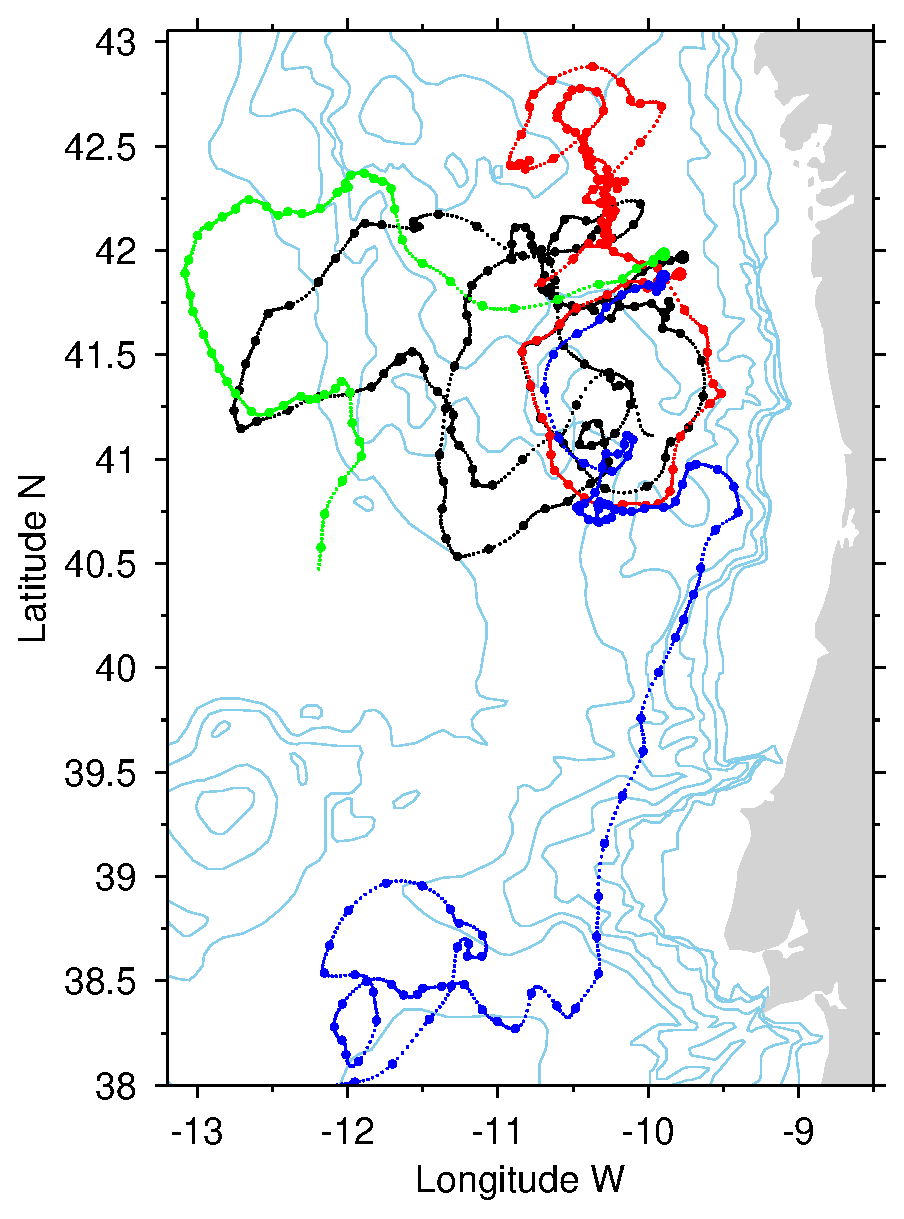
\includegraphics[width=7cm]{summerall}%
\caption{Summer deployment drifter tracks. Solid dots indicate
days. The minimum duration of the tracking was 60 days (green
drifter). Only data before the end
of 1998 are shown corresponding to 420 drifter days.} %
\label{fig:drf_summerall}
\end{figure}

In the summer deployment (Fig~\ref{fig:drf_summerall}), the four
drifters were released on 12 August 1998 in a cluster of 5nm side
square in the core of an upwelling filament previously identified
from SST images (see Chapter~\ref{ch:summer}). Minimum tracking
was 60 days, totaling 420 drifter days (see
Table~\ref{tb:drf_deploym}).

The summer period was a good representation of the upwelling
system with fully developed filaments and a broad band of upwelled
water extending beyond the shelf ($\sim$100km from the coast, see
Fig.~\ref{fig:cd114drf_sat}a). Three filaments were present at the
time of the deployment. The 42\deg N filament is the most
persistent one and reappears in the same location every year. The
northern most filament at 43\deg N was growing at the time but
shortly after the cruise faded away. The southern 41\deg N
filament was highly variable and underwent shifts in its location
that hindered its development. Overall, the drifters responded to
the changes of the system, slowing during a period of slack winds
and speeding up with increasing winds. Although filaments are
expected paths for exchange between shelf and open ocean only one
drifter traced the offshore extent of the SST signature of the
42\deg N filament and stayed offshore for 45 days prior to the end
of its transmission. The other drifters stayed in the filament
core before eventually crossing the filament southern boundary to
flow in an eddy like return flow onto the slope  with an average
velocity of 0.17$\pm$0.07\velc, which is of similar order to the
filament velocities. One of them then moved south along the shelf
break at a speed of 0.21$\pm$0.08 \velc. This southward flow was
related with the unusual extension of the upwelling season into
the autumn months. It left the shelf again near Cape Roca, a well
known site of filaments. The other two drifters stayed near their
original latitude of release with offshore excursions of
$\sim$100km before ending their transmission within 100km of the
coast.

In summary, the strongest flows were associated with the offshore
filament and the upwelling related slope southward flow. The
overall picture for the summer deployment is hence that of a rich
mesoscale field which actively links the shelf and the open ocean
at a large variety of time scales but with no clear net transport.


\subsection{Winter deployment}

In winter, westerly or southwesterly winds and northward flow  at
the slope like that described in Chapter~\ref{ch:winter} are
expected but exceptional weather gave conditions similar to
summer, therefore upwelling favourable. This situation was the
norm rather than the exception for the winter of 1999 as shown by
weekly averaged SST images spanning February-May 1999
(Fig~\ref{fig:drf_sst99}). No sustained poleward flow development
was evident in the SST in this period. Instead, a semi-permanent
coastal band of upwelled waters was identifiable in the images.
The only period of indicated poleward flow occurred during and
immediately after the winter deployment.

Overall, the winter deployment, made on 2 January 1999, showed a
remarkably different picture from the expected winter circulation.
Again the four drifters were released in a cluster of 5nm side
square but this time over the slope (1000m depth). Minimum
tracking duration was 25 days for the drifter which grounded south
of Finisterre. The data amount to 400 drifter days.

\begin{figure}
\centering \abajocap \subfigure[\mbox{Jan\,31-6\,1999}]{
\includegraphics[width=6.5cm]{ga990131-0206medfincol}}%
\subfigure[\mbox{Feb\,21-27\,1999}]{\includegraphics[width=6.5cm]{ga990221-0227medfincol}}
\subfigure[\mbox{Mar\,28-3\,1999}]{\includegraphics[width=6.5cm]{ga990328-0403medfincol}}%
\subfigure[\mbox{May\,23-29\,1999}]{\includegraphics[width=6.5cm]{ga990523-0529medfincol}}
\caption{Examples of SST during the 1999 winter. Note the absence
of the warm tongue indicative of poleward flow along the coast. }
\label{fig:drf_sst99}
\end{figure}
\begin{figure}
\centering %
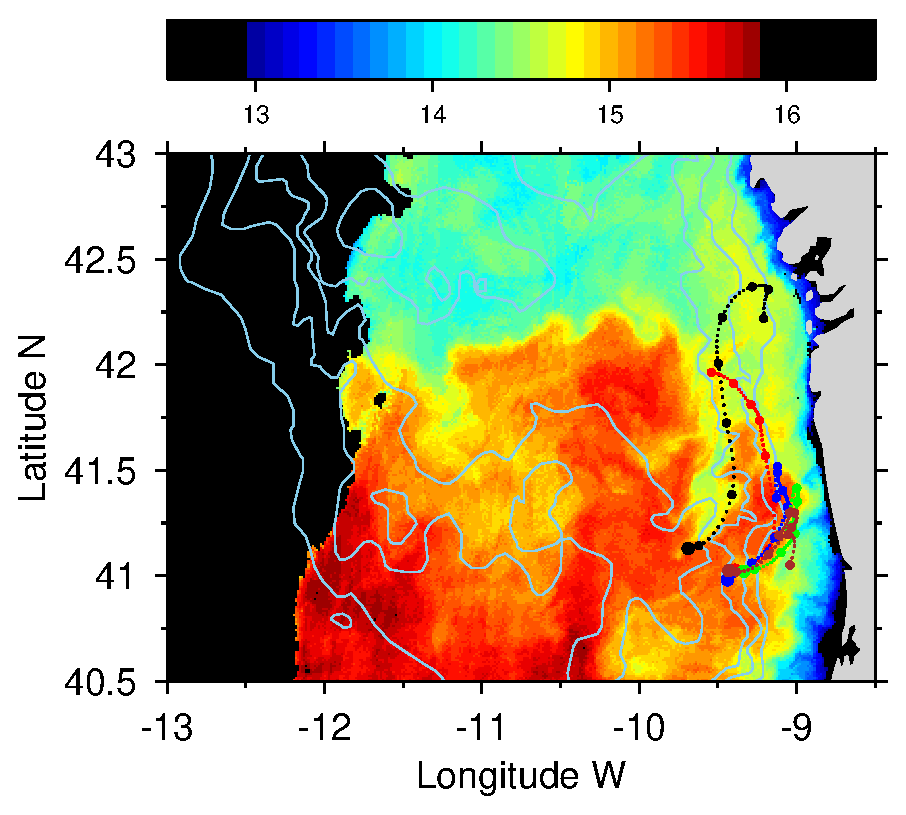
\includegraphics[width=7cm]{winterflow}%
\caption{Drifter data for the period 2-10 January 1999 overlaid on
the SST image of the 6 January 1999. Dots correspond to the start
of each day. Black corresponds to cloud masking.}
\label{fig:drf_pwflow}%
\end{figure}

The typical poleward flow over the slope described in
Chapter~\ref{ch:winter} was only present during early January
(Fig~\ref{fig:drf_pwflow}). The drifters, in the period 2-10
January moved northward following the bathymetry in a warm tongue
seen in SST image of 6 January. Velocity estimates from the
drifter positions give a mean value of 0.27$\pm$0.08 m/s similar
to the highest ADCP near surface velocity measured during the
winter cruise (Chapter~\ref{ch:winter}). Surface isobaric pressure
charts from the 11 January showed the onset of northerly winds and
the drifters ceased their northward motion. The warm slope anomaly
structure weakened during January as seen in SST images but was
nonetheless present until the end of January. The rest of the
winter deployment (Fig~\ref{fig:drf_winterall}) saw a net
southward flow both near and offshore  and there was a clear
inhibition of the shelf-ocean exchange seen during the summer
deployment. This arises from the upwelling favourable winds that
have been "typical" of the 1999 winter season. Mean velocity
estimates varied between 0.22 and 0.11 m/s. The offshore southward
flow is related to the Portugal Current, the easternmost branch of
the North Atlantic subtropical gyre, which showed mean velocities
of 0.17$\pm$0.08 m/s.

\begin{figure}
\centering %
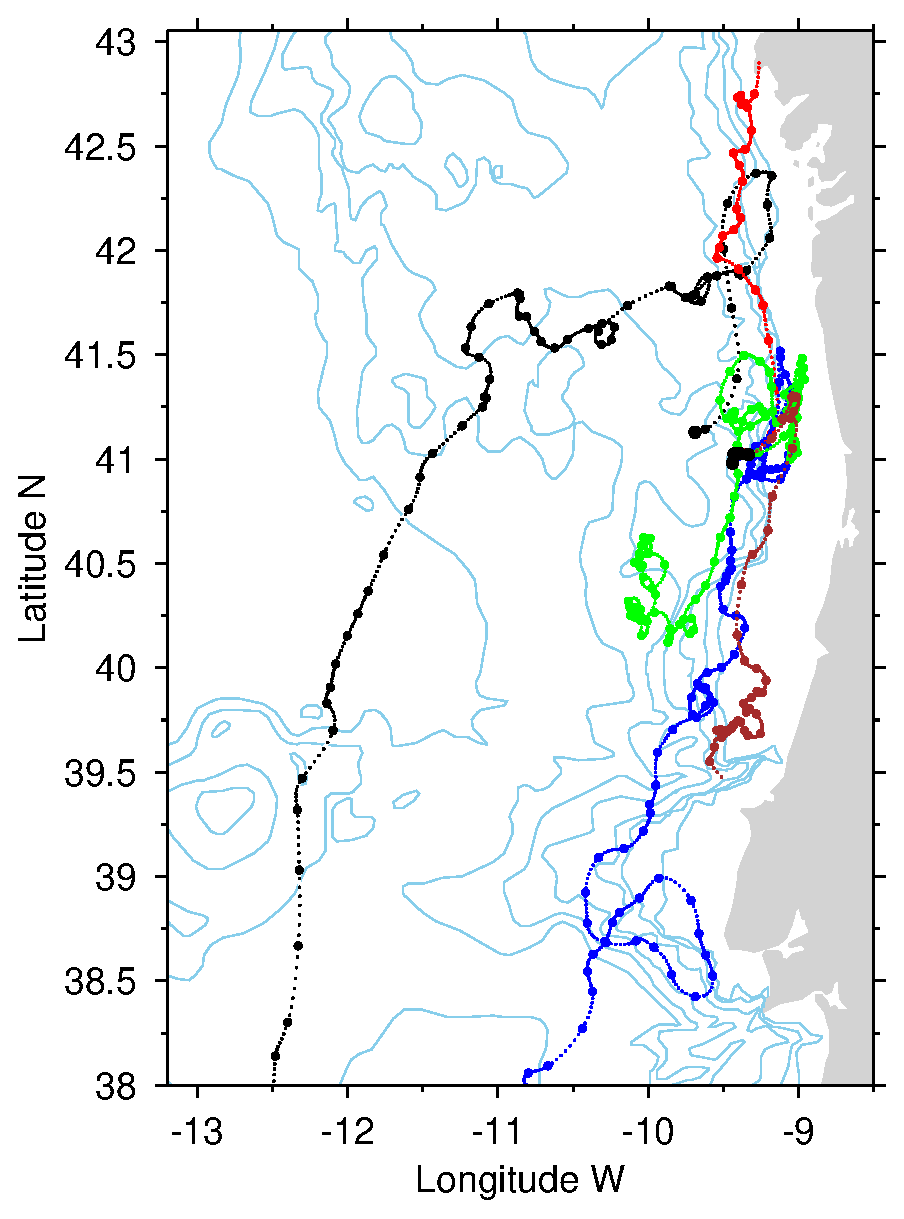
\includegraphics[width=7cm]{winterall}%
\caption{Winter deployment}%
\label{fig:drf_winterall}%
\end{figure}

\section{Lagrangian statistics and diffusivity estimates}

Lagrangian statistics were calculated for both deployments
following the method described in \citet{Davis85} and subsequently
used by many authors \citep[e.g.][]{Haynes91,Salas01}. Arriving to
statistically significant conclusions from Lagrangian measurements
requires the separation of the flow into mean and perturbation
components. The mean velocities ($U$,$V$, see
Table~\ref{tb:drf_drifters}) were obtained for each deployment and
subtracted from the calculated values to get the perturbation
components ($u'$,$v'$). To quantify the influence of the
perturbation flow on the mean flow we have to determine an eddy
diffusivity coefficient ($K$). To calculate it from Lagrangian
statistics it is usual to apply the theory of homogeneous
isotropic turbulence following the Taylor's Theorem
\citep{Taylor21}. A more complex approach was presented in
\citet{Davis87} and \citet{Davis91} where the diffusivity is not
assumed constant and where the flow homogeneity and infinitesimal
eddies constraints (infinitesimal eddies that are no longer
related to the mean flow, \emph{i.e.} at the end of the energy
cascade) are relaxed. This is basically a generalization to
circumstances with mean flow of the single-particle diffusivity
introduced by \citet{Taylor21}. However, the limited number of
drifters restricted its implementation.

Mean global velocities (Table~\ref{tb:drf_drifters}) indicated a
small southwestward drift during the summer deployment although
the values were not significantly different from zero. The winter
zonal average was again not different from zero but the meridional
component showed a small southward drift as seen in the drifter
trajectories.

Characteristic integral space and time scales can be defined from
the normalised autocorrelation function $R(\tau)$ of Lagrangian
velocity perturbation components $u',v'$ given by
\begin{equation}\label{eq:drf_R}
   R_{ij}(\tau) = \frac{1}{\overline{u_i'u_j'}T} \int^{T}_0
   u_i'(t)u_j'(t+\tau)dt,
\end{equation}
$T$ being the length of the time series, the overbar and ensemble
average and the subindices $i,j$ correspond to the zonal and
meridional components respectively. The Lagrangian integral
timescale $T_{ii}$ represents a measure of the time over which a
particle remembers its path. Its dependence on the autocorrelation
function $R(\tau)$, which is usually close to zero for long lags
($\tau$) but often exhibit a systematic trend of oscillations
(Fig~\ref{fig:drf_diff}), masks the evaluation of
Eq~\ref{eq:drf_Tl}. This is usually solved by time integrating the
velocity autocorrelation function $R(\tau)$ to the first zero
crossing $T_0$ giving an upper bounds limit \citep{Poulain89}.
\begin{equation}\label{eq:drf_Tl}
   T_{ii} = \int^{T_0}_0 R_{ii}(\tau)d\tau.
\end{equation}
The equivalent Lagrangian length scale $L_{ii}$ is defined
accordingly,
\begin{equation}\label{eq:drf_Ll}
   L_{ii} = \sqrt{\overline{u_i'^2}} \int^{T_0}_0
   R_{ii}(\tau)d\tau = \sqrt{\overline{u_i'^2}}T_{ii}.
\end{equation}
The small differences in each deployment between the two
components of $T_{ii,jj}$ and $L_{ii,jj}$
(Table~\ref{tb:drf_drifters}), support the initial isotropic
assumption implied in the analysis. Larger Lagrangian time and
space scales were obtained from the summer deployment and reflect
the larger, energetic features associated with the summer
upwelling, as $T$ and $L$ generally increase with the Eddy Kinetic
Energy (EKE) of the system \citep[i.e.][]{Martins02}.
\begin{figure}
\centering %
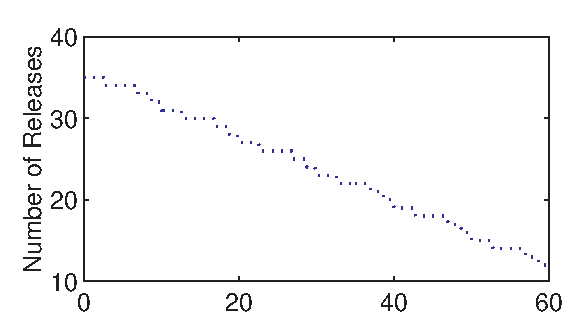
\includegraphics[width=7cm]{winter_rel}%
\caption{Number of ``new drifter'' releases for the winter
deployment. }
\label{fig:drf_releases}%
\end{figure}

\begin{table}
  \centering
\begin{tabular}{rrrrrrrrr}
\hline \hline & \multicolumn{2}{c}{ Velocity } &
\multicolumn{2}{c}{Time scale}& \multicolumn{2}{c}{Length scale}&
\multicolumn{2}{c}{Diffusivity}\\
\cline{1-9}  & $U$  & $V$  & $T_{ii}$ &
 $T_{jj}$ & $L_{ii}$ & $L_{jj}$  &
 $K_{ii}$ & $K_{jj}$\\
  & $cms^{-1}$  & $cms^{-1}$  & $days$ &
 $days$ & $km$ & $km$  & $10^6 cm^2s^{-1}$ & $10^6 cm^2s^{-1}$\\
 \cline{1-9} %
Summer&-1.45&-1.64&2.01&1.68&18.7&20.5&8.7&10.7\\
Winter&-1.42&-6.08&1.14&1.26&10.2&12.1&1.9&3.3\\
Global&-0.65&-2.21&1.41&1.57&12.5&15.9&5.2&10.6\\
\hline \hline
\end{tabular}
  \caption{Summary of bulk Lagrangian statistics for each of the
  deployments and of all available data, see text for details.}
  \label{tb:drf_drifters}
\end{table}

The number of drifters in each deployment (four) is insufficient
to arrive at statistically meaningful eddy diffusivity coefficient
estimates. Since the data set is assumed to be homogeneous and
stationary and the de-correlation time scale is small (maximum 2
days) it is common practise to increase the data set by generating
``new drifters'' every few $T_{ii}$
\citep{Colin83}(Fig.~\ref{fig:drf_releases}). By using a few
$T_{ii}$, the possibility of having unwanted correlations between
drifter segments which would corrupt the analysis is reduced. This
procedure allocates too much emphasis on the intermediate portions
of each trajectory, which is the most frequently sampled by this
segmentation process, and may constitute a disadvantage given the
small number of drifters. However, it is expected that the
increase in degrees of freedom compensates for this. For all
deployments, drifters were segmented every 10 days. The dispersion
of the segmented drifters (Fig~\ref{fig:drf_dye}, example from the
summer deployment) resembles the dispersion of an instantaneous
dye release about its center of gravity, highlighting the
diffusive character of the Iberian currents.

According to \citep{Taylor21}, the single-particle dispersion
(displacement variance) is related to the autocorrelation function
and the variance of their velocities:
\begin{equation}\label{eq:drf_disp}
   \overline{x'^{2}(t)} = \overline{2u'^{2}}\int^t_0(t-\tau)R_{ii}(\tau)d\tau
\end{equation}
where the bar indicates an ensemble average and $x'(t)$ is the
displacement of the particle due to $u'$ and $R_{ii}(\tau)$ is the
normalised autocorrelation coefficient of the perturbation
velocity.
\begin{figure}
\centering %
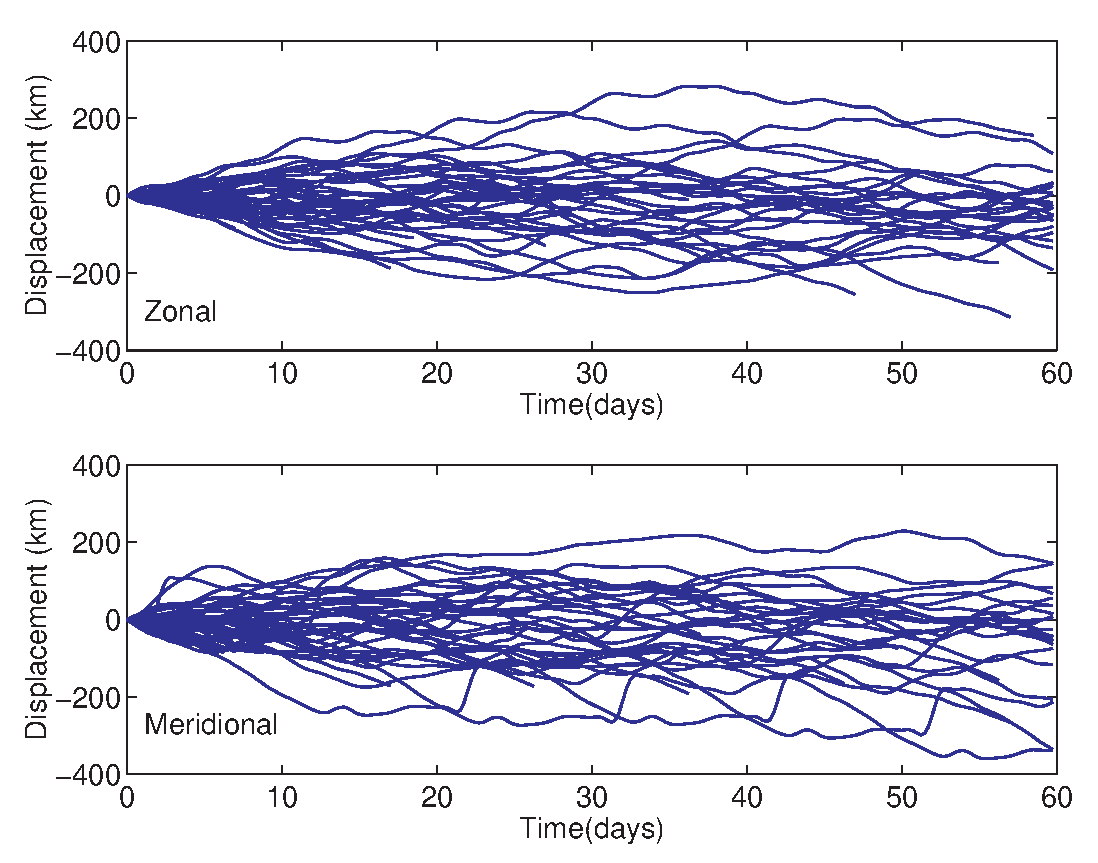
\includegraphics[width=7cm]{summer_plume}%
\caption{Example of displacement from each of the ``new released''
drifter segments from a single source. Note the similarity to a
diffusive dye plume.}
\label{fig:drf_dye}%
\end{figure}
Equation~\ref{eq:drf_disp} reaches two
asymptotic limits independent of the form of $R(\tau)$:\\
Initial dispersion, as $t\rightarrow 0$, $t<T$,
\begin{equation}\label{eq:drf_inidisp}
    \overline{x'^2}=\overline{u'^2}t^2,
\end{equation}
and Random walk regime for $t\gg T$,
\begin{equation}\label{eq:drf_randw}
    \overline{x'^2}=\overline{2u'^2}Tt.
\end{equation}
The Lagrangian diffusivity is then defined as half the rate of
change of the dispersion. Equation~\ref{eq:drf_diff} allows
diffusivities to be calculated in two ways: by directly evaluating
the derivative of the left-hand side, and the other by numerical
integration of the right-hand side. The result presented here were
arrived at through the second method.
\begin{equation}\label{eq:drf_diff}
    K_{ii} = \frac{1}{2} \frac{\overline{dx'^2}}{dt}=\overline{u'^2}
    \int^{T_0}_0 R_{ii}(\tau) d\tau = \overline{u'^2}T_{ii}.
\end{equation}
\begin{figure}
\centering %
\subfigure[]{
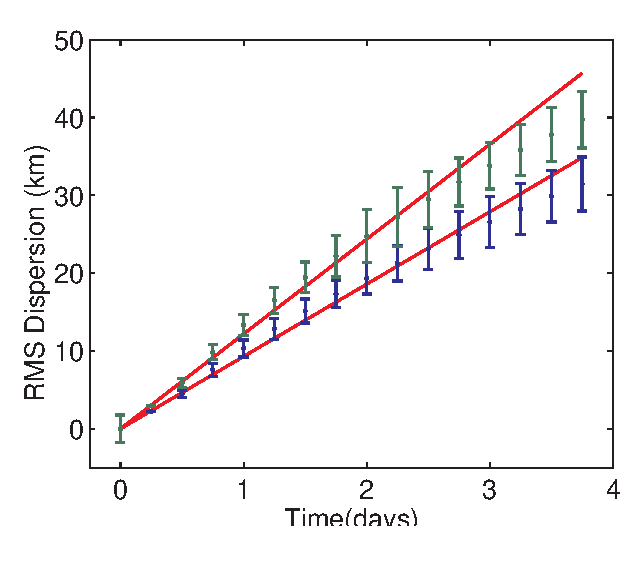
\includegraphics[width=5cm,trim=0 0 0 -30,clip]{summer_inidisp}}
\subfigure[]{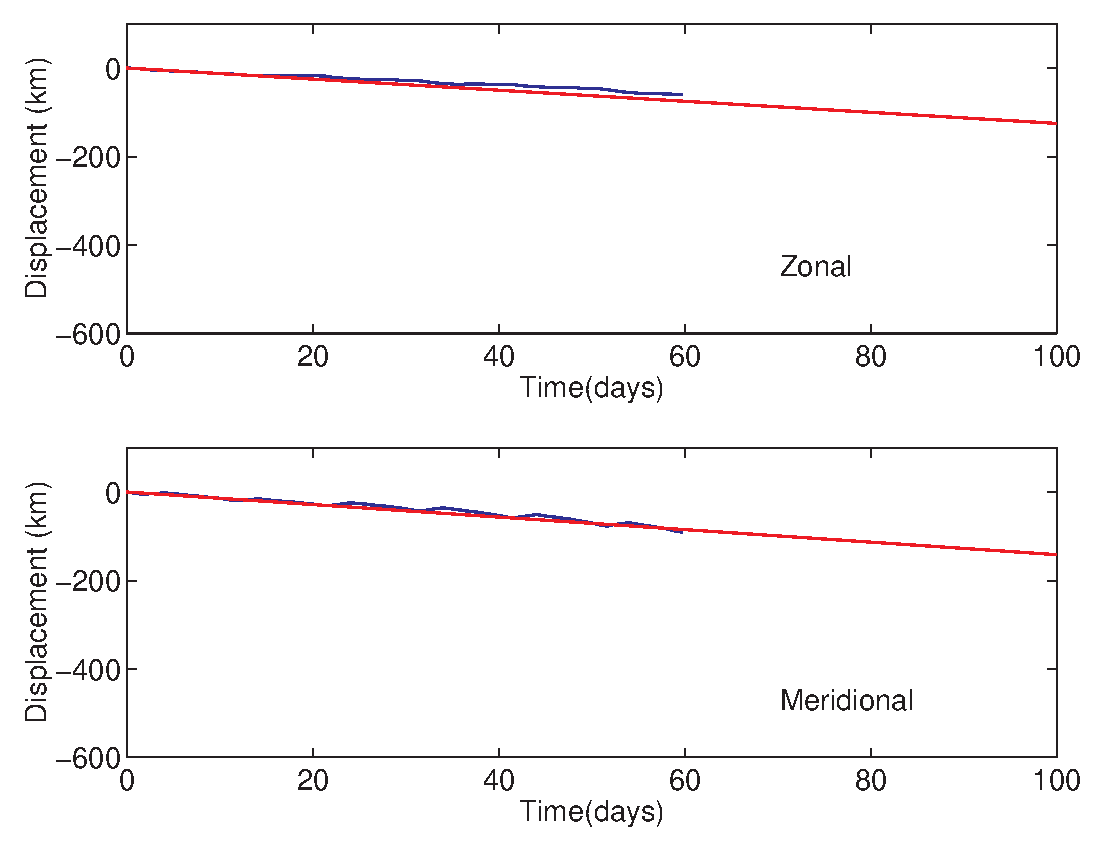
\includegraphics[width=7cm,origin=c]{summer_meandisp}}
\caption{Examples of Taylor assumptions evaluation for the summer
deployment. a) Initial displacement and b) mean displacement.}
\label{fig:drf_dispcomp}%
\end{figure}
The validity of Taylor's Theorem ( and hence our assumptions of
homogeneity and stationarity ) can be assessed by comparing the
data against the theoretical initial dispersion and the final
random walk regime. Calculated Taylor's initial dispersion is
overlaid on the summer observed root mean square (RMS) dispersion
together with error bands (Fig.~\ref{fig:drf_dispcomp}a, green for
meridional and blue for zonal). Both data agree for the first 2
days hence giving further support to the applicability of Taylor's
Theorem in the OMEX region. Similar agreement was found for the
winter deployment. Mean displacements of the segmented data
(Fig.~\ref{fig:drf_dispcomp}b) agree well with the values of the
removed background mean flow which supports our assumption that
the flow field can be approximated by the Taylor theorem (example
from the summer deployment).

The time evolution of  the RMS dispersion of the summer drifters
(Fig~\ref{fig:drf_summerrms}a, blue is zonal and green is
meridional) shows an rapid increase in dispersion corresponding to
the initial Taylor dispersion. After that, dispersion is highly
reduced and maintained constant for 30 days reaching the linear
random walk regime only in the last part of the record. This
behaviour might be characteristic of upwelling-filament areas
where the bulk dispersion will largely depend on the time scales
under consideration. The log-log plots\begin{figure}
\centering %
\subfigure[]{
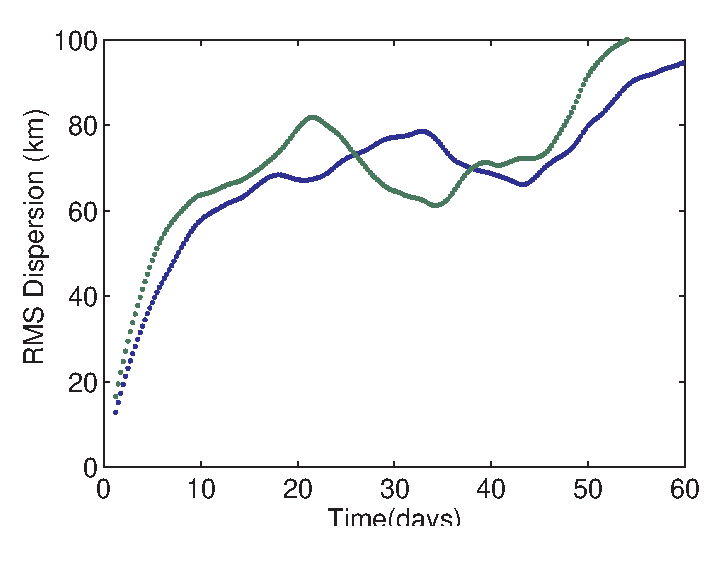
\includegraphics[width=5cm,trim=0 0 0 -45,clip]{summer_rmsdis}}
\subfigure[]{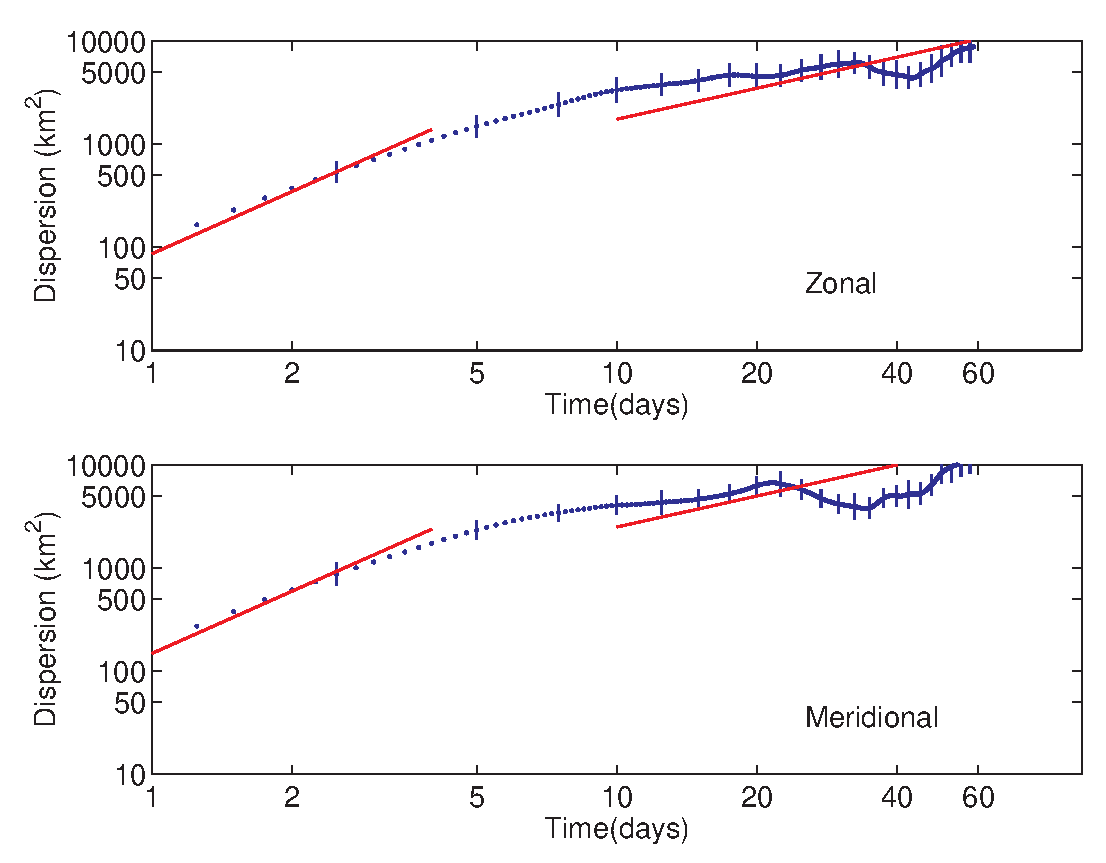
\includegraphics[width=7cm]{summer_logdisp}}
\caption{Displacement plots for summer deployment. a) RMS
displacement and b) Log-Log zonal (top) and meridional (bottom)
dispersion. Symbols represent observations,  solid lines represent
Taylor's theorem for initial dispersion and random walk regime.
Error bars represent 67\% confidence.}
\label{fig:drf_summerrms}%
\end{figure}
(Fig.~\ref{fig:drf_summerrms}b) of zonal (top) and meridional
(bottom) summer dispersion versus time again shows the agrement
with Taylor's theorem of initial dispersion. The Random Walk
regime agreement is worse possibly due to the large effect of
eddies in the dispersion. Error bars represent 67\% confidence
limits of the dispersion.

The winter RMS dispersion (Fig~\ref{fig:drf_winterrms}a) is much
smaller than in summer with the two regimes (Initial and Random
Walk) clearly distinctive. The differences between zonal (green)
and meridional (blue) RMS dispersion are more significant due to
the more anisotropic diffusive winter regime. The agreement
between the Random Walk regime and the observations
(Fig~\ref{fig:drf_winterrms}b) is now better. Comparing the
drifter's behaviour during summer and winter
(Fig.~\ref{fig:drf_winterrms}a-b) one can note that there is a
much higher initial dispersion during the summer associated with
the large-scale eddy identified in the drifter tracks.

Summer and winter diffusivities and the autocorrelation function
for both zonal and meridional components are shown in
Fig.~\ref{fig:drf_diff}. The diffusivities were calculated by
integrating the autocorrelation function. The final value is the
average of the diffusivity over the time when it approaches a
constant value. They are expected to asymptote at a few $T_{ii}$
and failing to do so manifests the difficulties in estimating
$K_{ii}$ from a limited amount of drifter data. Winter
diffusivities did indeed approach a constant value in a few
$T_{ii}$, from day 20, giving support to the assumptions of
stationary and homogeneity, with averages of $1.9\times10^2$\mix
and $3.3\times10^2$\mix in the zonal and meridional components.
\begin{figure}
\centering %
\subfigure[]{
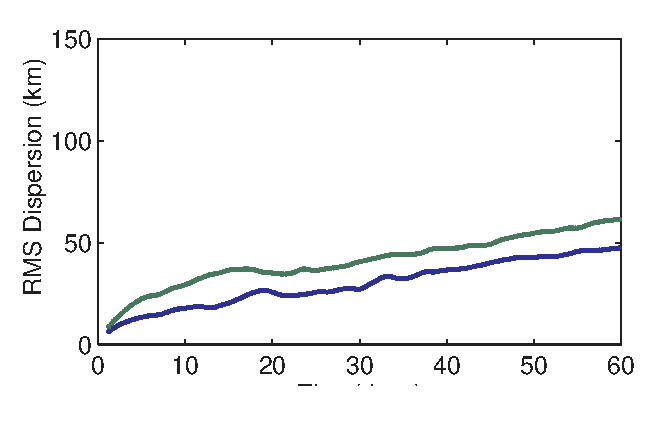
\includegraphics[width=6cm,trim=0 0 0 -45,clip]{winter_rmsdisp}}
\subfigure[]{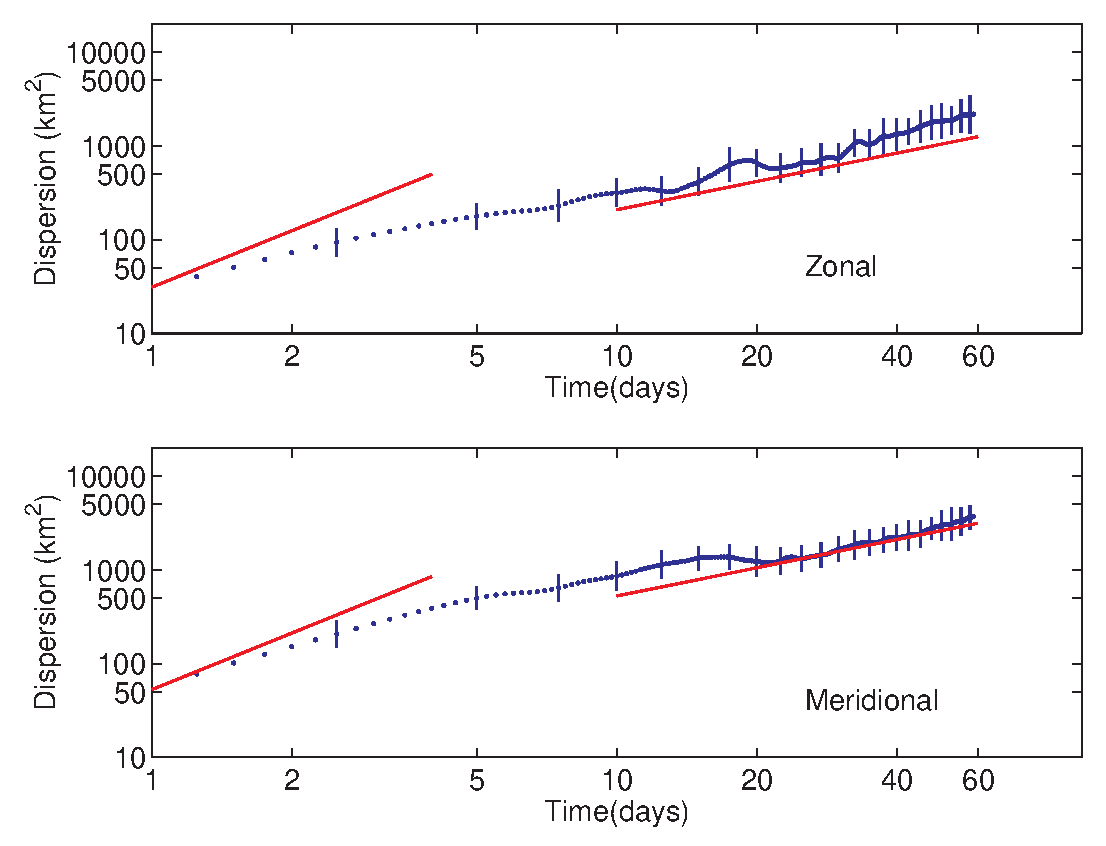
\includegraphics[width=7cm]{winter_logdis}}
\caption{Displacement plots for winter deployment. a) RMS
displacement against time and b) Log-Log zonal (top) and
meridional (bottom) dispersion. Symbols represent observations,
solid lines represent Taylor's theorem for initial dispersion and
random walk regime. Error bars represent 67\% confidence.}
\label{fig:drf_winterrms}%
\end{figure}
Summer diffusivities were much higher and failed to asymptote
until day 50 suggesting that the inhomogeneities in the flow were
large. Final averages suggest small isotropy with values of
$8.7\times10^2$\mix (zonal) and $10.7\times10^2$\mix (meridional).
The number of drifters decrease with time and summer diffusivities
should be taken with caution as sampling errors increase. It is
worth mentioning the sharp peak in the diffusivity at times
smaller than 10 days. This is caused by the presence of the
eddy/filament meander as mentioned previously. Similar results
were obtained by \citet{Swenson96} for drifters deployed in the
California Current system in regions where eddies were present.


\begin{figure}
\centering %
\subfigure[]{
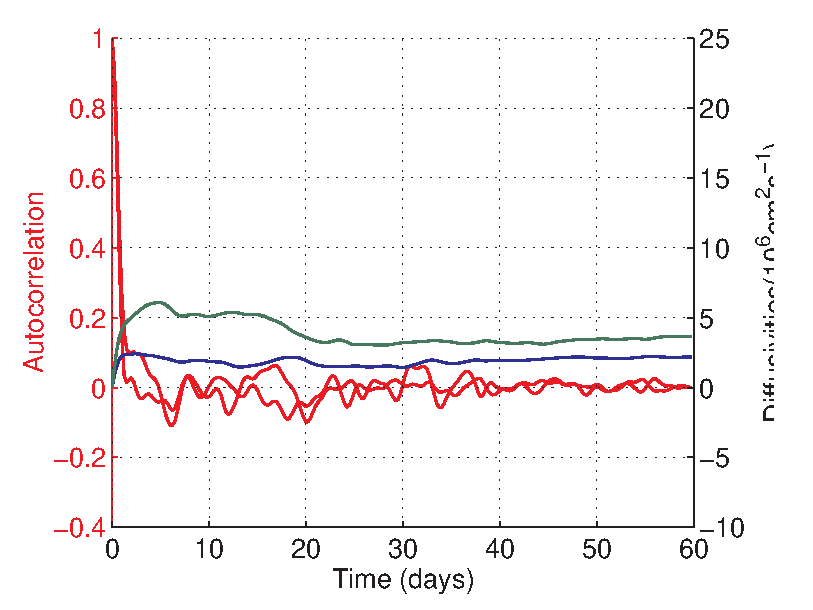
\includegraphics[width=7cm,trim=0 0 0 -13,clip]{winter_diff}}
\subfigure[]{\includegraphics[width=7cm]{summer_diff}}
\caption{Diffusivity and autocorrelation function with time for
the, a) summer and b) winter deployments for both zonal (blue) and
meridional (green) components.}
\label{fig:drf_diff}%
\end{figure}

The analysis was repeated with all available mixed layer drifters
for the region including data from a previous deployment in autumn
1986. During that time the drifters moved northward following the
winter poleward slope in contrast with our winter data. A full
description of the data can be found in \citet{Haynes91}. The bulk
results show a better agreement with Taylor's theorem
(Fig~\ref{fig:drf_allrms}) due to the larger number of
realisations. The number of ``pseudo drifters'' decreases linearly
from 150 to 50 at day 90. The dispersion versus time graph
(Fig~\ref{fig:drf_allrms}a) shows clearly the two regimes. In this
final case, differences between zonal and meridional components
have increased with respect to the winter and summer values.The
Log-Log plots (Fig~\ref{fig:drf_allrms}b) also show a better
agreement between observations and Taylor's theorem than in the
separate deployments.
\begin{figure}
\centering %
\subfigure[]{
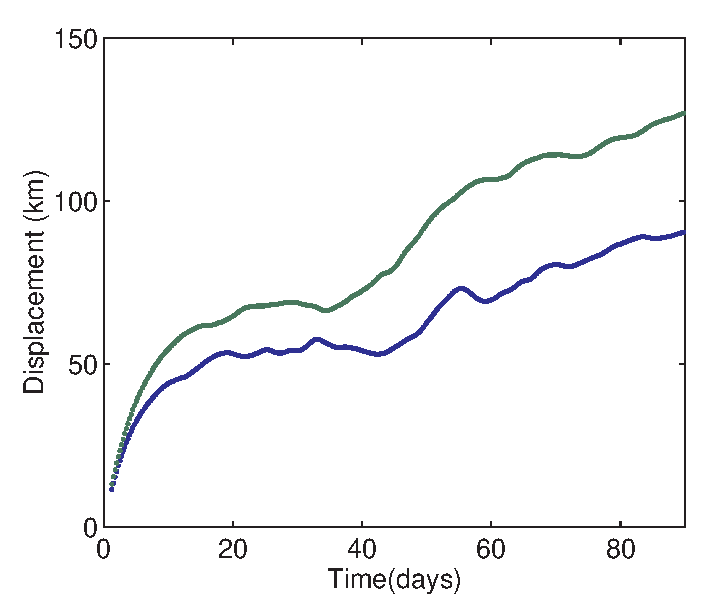
\includegraphics[width=6cm]{all_disp}}
\subfigure[]{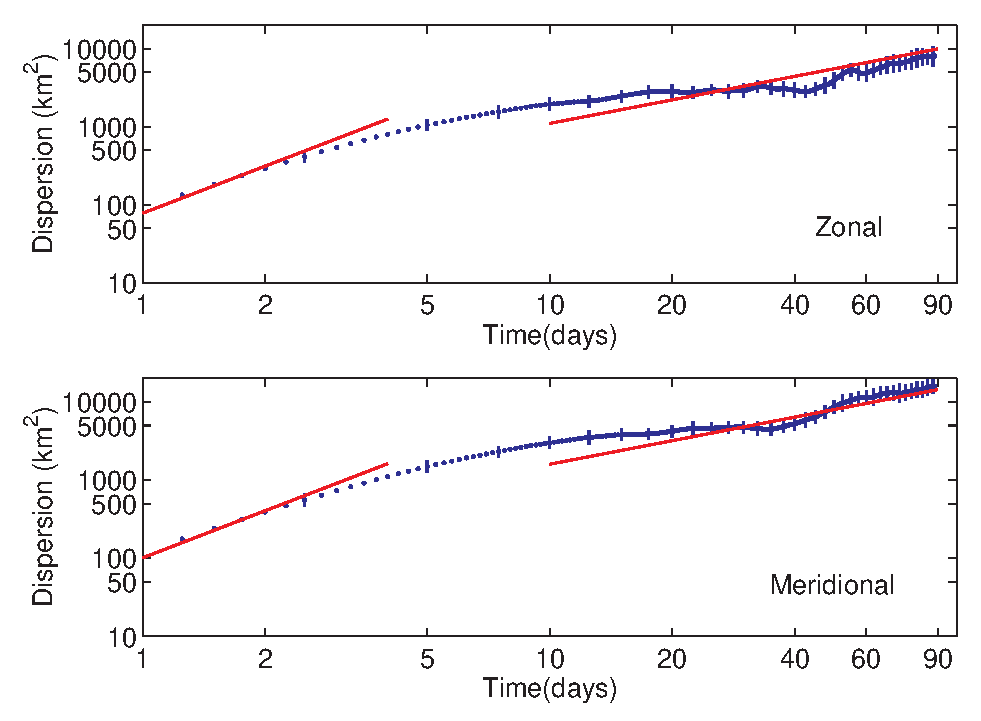
\includegraphics[width=7cm]{all_logdis}}
\caption{Displacement plots for all available data. a) RMS
displacement against time and b) Log-Log zonal (top) and
meridional (bottom) dispersion. Symbols represent observations,
solid lines represent Taylor's theorem for initial dispersion and
random walk regime.}
\label{fig:drf_allrms}%
\end{figure}

The bulk Lagrangian length scales were 12.5km and 15.9km for the
zonal and meridional directions, which lay in between the values
for the two seasons. The Lagrangian time scales were 1.41 days
(zonal) and 1.57 days (meridional). The diffusivities and
autocorrelation function (Fig~\ref{fig:drf_alldiff}) shows
characteristics from the summer deployment. The diffusivity peaks
similarly to the summer deployment and asymptotes around day 50.
The final averages were also a compromise between the two seasons
with values of $5.2\times10^2$\mix (zonal) and
$10.6\times10^2$\mix (meridional) although they became more
anisotropic.

\begin{figure}
\centering %
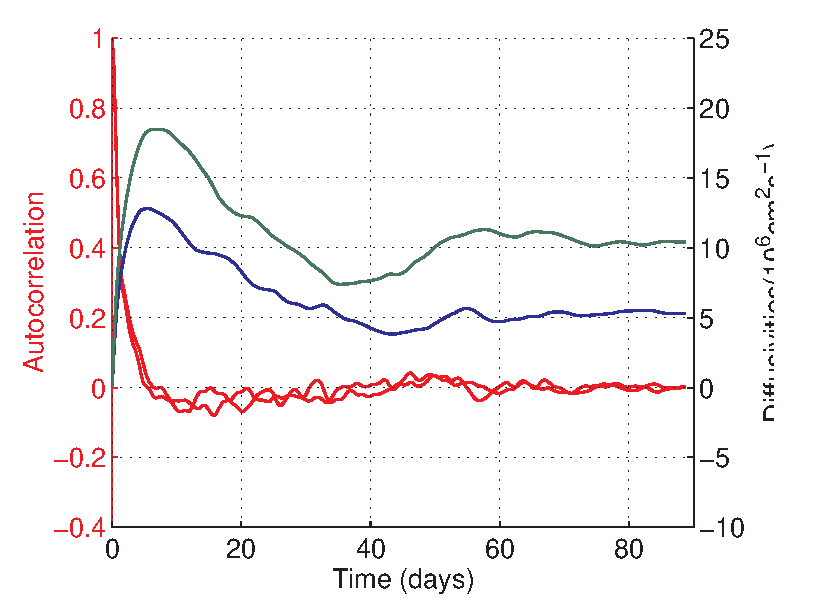
\includegraphics[width=7cm]{all_diff}
\caption{Diffusivity and autocorrelation function with time
calculated from all available drifter data for both zonal (blue)
and meridional (green) components.}
\label{fig:drf_alldiff}%
\end{figure}

The relationship between estimates of $K$ and the EKE of the
system is explored in Figure~\ref{fig:drf_diffeke}. The current
data is plotted alongside to previously published data extracted
from \citet[][and references therein]{Martins02}. The data
includes other upwelling areas like the California Current and
oceanic regions like the North Atlantic or Azores regions. As
expected a general trend is observed, with regions or seasons of
larger EKE having larger $K$. The current $K$ estimates are the
smallest. In our limited dataset a clear increase in EKE and $K$
can be seen from winter to summer which is also supported by the
data from \citet{Haynes91}.
\begin{figure}
\centering %
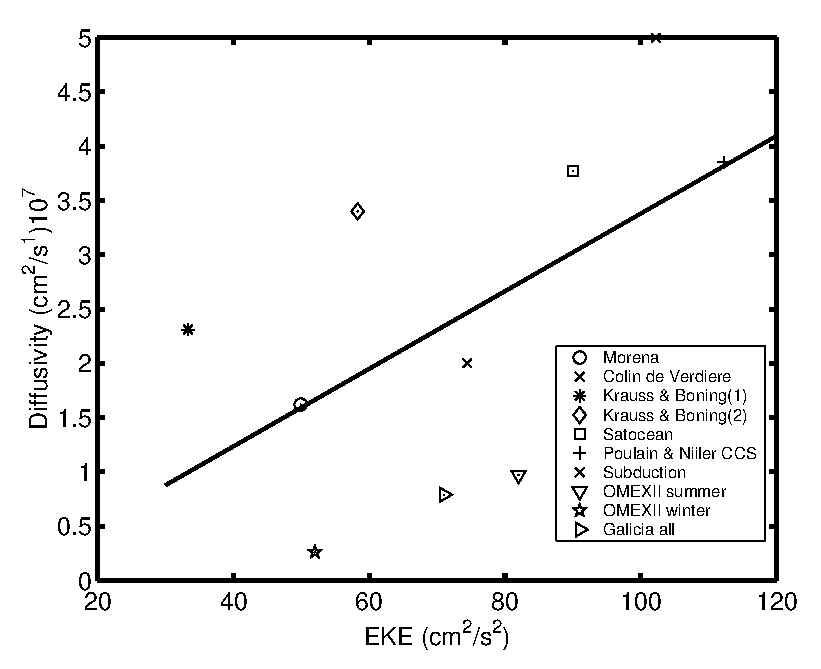
\includegraphics[width=7cm]{diffeke}
\caption{Diffusivity against EKE for the current data and other
published data extracted from \emph{Martins et al.,}[2002]. See
text for details.}
\label{fig:drf_diffeke}%
\end{figure}



\section{Discussion}
This chapter has aimed to quantify the observed variability of
summer and winter regimes in terms of the Eddy diffusivity as
estimated from drifter data. Although the dataset is small it was
shown to conform to Taylor's theorem and the single-particle
diffusivity method is expected to be of significance. Validity of
the method with this small number of drifters should however be
viewed with caution. In order to obtain more reliable estimates
data were searched for in the WOCE drifter database but the other
deployment documented there (from the MORENA project) did not have
public access to the data.

Nonetheless there are limitations and associated errors that
should be considered. First of all, our limited number of drifters
means that the spatial coverage was limited and unevenly sampled.
This adds an intrinsic bias in $K$ estimates towards high
diffusivity areas. This is proportional to the mean gradient of
particle concentration, which can be solved by using spatial
ensembles of uniform average buoy density for which a much larger
and extensive deployment strategy should be used. The velocity
departure normalised by the variance should fit a Gaussian
distribution for the single-particle method to be applicable. It
was found that the distribution of all available data was always
marginally different from Gaussian (Fig~\ref{fig:drf_hist}),
although more so for the meridional component. This could be
accounted for by spatial inhomogeneity, more so during the summer,
and the presence of the coast.

\begin{figure}
\centering %
\subfigure[]{
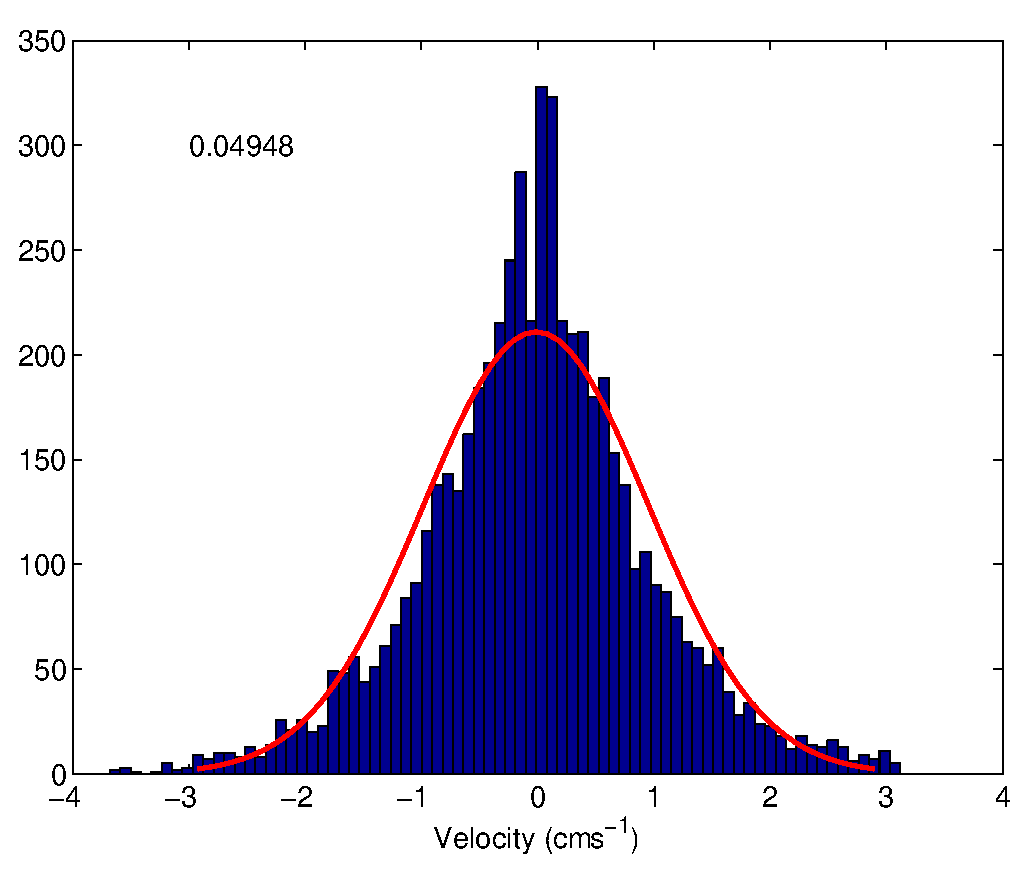
\includegraphics[width=6cm]{Ugauss}}
\subfigure[]{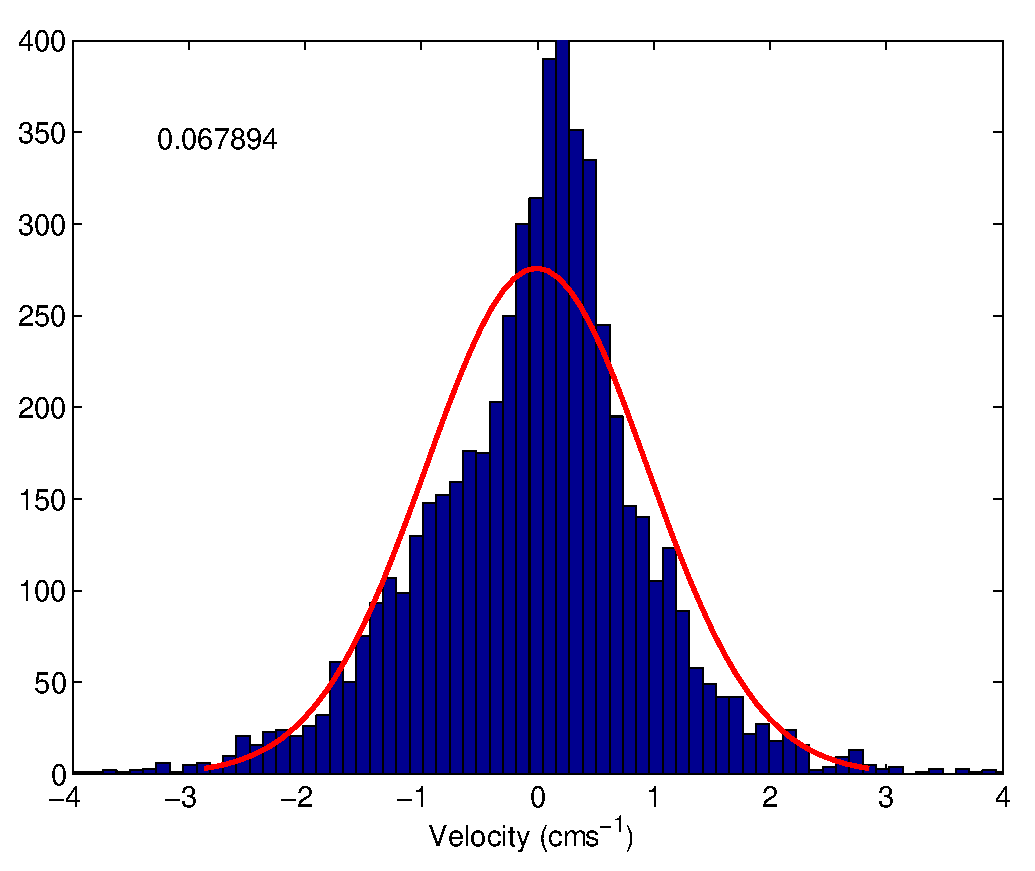
\includegraphics[width=6cm]{Vgauss}}
\caption{Histograms for the global analysis of velocity departure
statistics for the zonal (a) and meridional (b) components
normalised by the observed variance. The red line is the fitted
Gaussian distribution. The number in the upper left-hand corner of
each figure is the Kolmogorov-Smirnov statistical test value for
normal distribution. Values smaller than 0.0179 means the data is
normal distributed. Although they are not gaussian distributed at
the 95.5\% level of confidence, the zonal component is closer to a
Gaussian distribution than the meridional one.}
\label{fig:drf_hist}%
\end{figure}
Although weather conditions proved to be very similar during the
two deployments there are clear differences in drifter behaviour
in the summer and winter periods. The activity of upwelling
filaments marks the summer surface circulation and they act as an
active link between the shelf and open ocean but the associated
return flow inhibits a net offshore flow of shelf waters
\citep{Barton01}. During winter, filaments did not occur, even
though upwelling conditions persisted, and shelf waters were
isolated from the ocean. During this exceptional winter, there has
been a net southward transport over the slope contrary to previous
evidence of persistent winter poleward flow.

We have found clear differences in the Lagrangian statistics of
the two deployments, summer and winter, although they cannot
solely be attributed to seasonal differences. The summer drifters
stayed mostly offshore away from the constraint of the coast and
one expects the regime to be more isotropic
\citep[e.g.][]{Martins02}. The larger scales of the dominant
physical processes (filaments and eddies) caused the
diffusivities, Lagrangian length and time scales to be bigger
during the summer. The winter drifters stayed mostly close to the
coast, which made the diffusivity slightly anisotropic. Also, the
physical processes involved were weaker and no signs of eddy
formation were seen, which is characteristic of the winter
circulation in the Iberian Coastal Transition Zone
\citep{Haynes91,Huthnance02}. Overall, the diffusivities and
Lagrangian scales were smaller. One has to be however careful in
interpreting the winter data as dispersion in the slope region in
the presence of the slope current is critically dependent on the
initial deployment position relative to the slope current
\citep{Burrows99}. The 1986 deployment of \citet{Haynes91} was
done under typical winter conditions with a well developed
poleward flow and evidences of eddy shedding from it.
Nevertheless, their values of diffusivity ($3.4\times10^2$\mix and
$2.5\times10^2$\mix for zonal and meridional), Lagrangian length
scale (9.2 and 11.2km) and time scale (1.3 and 1.9 days) were
similar to our winter deployment. The main discrepancies were
found in the zonal values were the eddies acted to increase these
scales. \citet{VanAken02} found larger eddy activity in the Bay of
Biscay during the poleward flow regime, an extension of the
Portugal poleward flow, in drifter data but the region lacks the
summer upwelling regime so comparisons can not be easily drawn.
Although slope water eddies are believed to play a significant
role in the shelf-ocean exchange during the winter
\citep{Huthnance02} they are not continuously generated at any
location (although there are preferred sites) and export bulk
capabilities remain to be assessed.

One of the main difference between the summer and winter
deployments is the shape of $K(t)$, which sharply peaks in the
summer one as a consequence of the strong eddy like signals in the
tracks. Similar results were also observed by \citet{Swenson96}
induced by relevant spatial inhomogeneity.

\section{Conclusions}
It was expected that there would be a seasonal modulation of the
Lagrangian statistics in the Iberian CTZ mainly due to the
seasonality of the currents regime. However, the present data
lacks sufficient spatial coverage during either season to
determine the amount of our temporal variation due to spatial
differences and the proportion due to seasonal changes.
Nonetheless we can conclude that:
\begin{itemize}
\item Clear differences were seen in the drifter behaviour during
the two deployments despite the similar atmospheric forcing
conditions.
\item During the summer, high values of EKE were found, and the
characteristic Lagrangian and time scales were larger than in the
winter deployment.
\item Diffusivity estimates were also larger during the summer than
during the winter deployment suggesting an increased mixing during
active upwelling and filament formation.
\item Diffusivity estimates compared well with previous estimates
in the region but rank in the lower end of estimates in other
upwelling areas.
\item Inclusion of all available data in the analysis showed a
better agreement with Taylor's theorem suggesting that more
drifter deployments are needed to accurately describe the
diffusivity seasonality in the region.
\item Diffusivity estimates from all available data were highly
anisotropic.
\end{itemize}

Despite its shortcomings, this work is important because of the
lack of observations in the area. Hopefully, with more deployments
there will be a better estimate of the eddy flux transport in the
region during the different regimes.
